\documentclass[11pt]{article}

% Reproducible PDF bytes: no creation date, no random trailer identifier, no producer banner.
\pdfinfoomitdate=1
\pdftrailerid{}
\pdfsuppressptexinfo=-1

\usepackage[letterpaper,margin=1in]{geometry}
\usepackage[T1]{fontenc}
\usepackage[utf8]{inputenc}
\DeclareUnicodeCharacter{2212}{\ensuremath{-}}
\usepackage{mathptmx}
\usepackage[scaled=0.92]{helvet}
\usepackage{microtype}
\usepackage{amsmath,amssymb}
\usepackage{booktabs,tabularx,array}
\usepackage[font=small,labelfont=bf,skip=4pt]{caption}
\usepackage{enumitem}
\usepackage{float}
\usepackage[section]{placeins}
\usepackage{pgfplots}
\usetikzlibrary{positioning,arrows.meta}
\pgfplotsset{compat=1.18}
\usepackage[numbers,sort&compress]{natbib}
\usepackage[hidelinks,pdftitle={From the tens digit to the suffix: token boundaries, early attention and a late decision in how small language models choose ordinal suffixes},pdfauthor={},pdfcreator={},pdfproducer={}]{hyperref}
\usepackage[nameinlink,capitalise]{cleveref}

\setlist{itemsep=2pt,topsep=3pt,parsep=0pt}
\setlength{\parskip}{3pt}
\setlength{\emergencystretch}{2em}
\renewcommand{\arraystretch}{1.12}
\newcolumntype{Y}{>{\raggedright\arraybackslash}X}
\crefname{appendix}{Appendix}{Appendices}

% Every number from the saved outputs is a macro generated from those outputs by a script.
% Generated by scripts/make_numbers.py from saved outputs. Do not edit.
% Use in the text as \nv{key}; an unknown key stops the build.
\expandafter\def\csname nv@c.gpt2.boundary.acct\endcsname{0.113}
\expandafter\def\csname nv@c.gpt2.boundary.auroc\endcsname{0.369}
\expandafter\def\csname nv@c.gpt2.boundary.hi\endcsname{0.465}
\expandafter\def\csname nv@c.gpt2.boundary.lo\endcsname{0.279}
\expandafter\def\csname nv@c.gpt2.boundary.nend\endcsname{2,920}
\expandafter\def\csname nv@c.gpt2.boundary.nnum\endcsname{10}
\expandafter\def\csname nv@c.gpt2.boundary.nteen\endcsname{80}
\expandafter\def\csname nv@c.gpt2.control.acct\endcsname{0.950}
\expandafter\def\csname nv@c.gpt2.control.auroc\endcsname{0.943}
\expandafter\def\csname nv@c.gpt2.control.hi\endcsname{0.965}
\expandafter\def\csname nv@c.gpt2.control.lo\endcsname{0.917}
\expandafter\def\csname nv@c.gpt2.control.nend\endcsname{200}
\expandafter\def\csname nv@c.gpt2.control.nnum\endcsname{138}
\expandafter\def\csname nv@c.gpt2.control.nteen\endcsname{200}
\expandafter\def\csname nv@c.gpt2.gap\endcsname{0.574}
\expandafter\def\csname nv@c.npass\endcsname{14}
\expandafter\def\csname nv@c.ntests\endcsname{14}
\expandafter\def\csname nv@c.ol.3.base\endcsname{6.24}
\expandafter\def\csname nv@c.ol.3.bauroc\endcsname{0.998}
\expandafter\def\csname nv@c.ol.3.kept\endcsname{0.995}
\expandafter\def\csname nv@c.ol.3.rmax\endcsname{1.007}
\expandafter\def\csname nv@c.ol.3.rmin\endcsname{0.989}
\expandafter\def\csname nv@c.ol.3.s00\endcsname{0.999}
\expandafter\def\csname nv@c.ol.3.s05\endcsname{0.997}
\expandafter\def\csname nv@c.ol.3.s09\endcsname{0.997}
\expandafter\def\csname nv@c.ol.4.base\endcsname{1.21}
\expandafter\def\csname nv@c.ol.4.bauroc\endcsname{0.768}
\expandafter\def\csname nv@c.ol.4.kept\endcsname{0.110}
\expandafter\def\csname nv@c.ol.4.rmax\endcsname{1.047}
\expandafter\def\csname nv@c.ol.4.rmin\endcsname{0.921}
\expandafter\def\csname nv@c.ol.4.s00\endcsname{0.781}
\expandafter\def\csname nv@c.ol.4.s05\endcsname{0.608}
\expandafter\def\csname nv@c.ol.4.s09\endcsname{0.724}
\expandafter\def\csname nv@c.ol.5.base\endcsname{3.71}
\expandafter\def\csname nv@c.ol.5.bauroc\endcsname{0.995}
\expandafter\def\csname nv@c.ol.5.kept\endcsname{0.993}
\expandafter\def\csname nv@c.ol.5.rmax\endcsname{1.020}
\expandafter\def\csname nv@c.ol.5.rmin\endcsname{0.994}
\expandafter\def\csname nv@c.ol.5.s00\endcsname{1.004}
\expandafter\def\csname nv@c.ol.5.s05\endcsname{0.994}
\expandafter\def\csname nv@c.ol.5.s09\endcsname{1.001}
\expandafter\def\csname nv@c.ol.7.base\endcsname{0.62}
\expandafter\def\csname nv@c.ol.7.bauroc\endcsname{0.651}
\expandafter\def\csname nv@c.ol.7.kept\endcsname{0.076}
\expandafter\def\csname nv@c.ol.7.rmax\endcsname{1.031}
\expandafter\def\csname nv@c.ol.7.rmin\endcsname{0.856}
\expandafter\def\csname nv@c.ol.7.s00\endcsname{0.715}
\expandafter\def\csname nv@c.ol.7.s05\endcsname{0.629}
\expandafter\def\csname nv@c.ol.7.s09\endcsname{0.745}
\expandafter\def\csname nv@c.olmo.3p.acce\endcsname{0.980}
\expandafter\def\csname nv@c.olmo.3p.acct\endcsname{1.000}
\expandafter\def\csname nv@c.olmo.3p.auroc\endcsname{1.000}
\expandafter\def\csname nv@c.olmo.3p.hi\endcsname{1.000}
\expandafter\def\csname nv@c.olmo.3p.lo\endcsname{0.999}
\expandafter\def\csname nv@c.olmo.3p.nnum\endcsname{7}
\expandafter\def\csname nv@c.olmo.4c.acce\endcsname{0.880}
\expandafter\def\csname nv@c.olmo.4c.acct\endcsname{0.965}
\expandafter\def\csname nv@c.olmo.4c.auroc\endcsname{0.989}
\expandafter\def\csname nv@c.olmo.4c.hi\endcsname{0.996}
\expandafter\def\csname nv@c.olmo.4c.lo\endcsname{0.979}
\expandafter\def\csname nv@c.olmo.4c.nnum\endcsname{71}
\expandafter\def\csname nv@c.olmo.4p.acce\endcsname{0.975}
\expandafter\def\csname nv@c.olmo.4p.acct\endcsname{0.220}
\expandafter\def\csname nv@c.olmo.4p.auroc\endcsname{0.775}
\expandafter\def\csname nv@c.olmo.4p.hi\endcsname{0.825}
\expandafter\def\csname nv@c.olmo.4p.lo\endcsname{0.722}
\expandafter\def\csname nv@c.olmo.4p.nnum\endcsname{71}
\expandafter\def\csname nv@c.olmo.5c.acce\endcsname{0.900}
\expandafter\def\csname nv@c.olmo.5c.acct\endcsname{0.940}
\expandafter\def\csname nv@c.olmo.5c.auroc\endcsname{0.974}
\expandafter\def\csname nv@c.olmo.5c.hi\endcsname{0.987}
\expandafter\def\csname nv@c.olmo.5c.lo\endcsname{0.959}
\expandafter\def\csname nv@c.olmo.5c.nnum\endcsname{169}
\expandafter\def\csname nv@c.olmo.5p.acce\endcsname{0.840}
\expandafter\def\csname nv@c.olmo.5p.acct\endcsname{1.000}
\expandafter\def\csname nv@c.olmo.5p.auroc\endcsname{0.999}
\expandafter\def\csname nv@c.olmo.5p.hi\endcsname{1.000}
\expandafter\def\csname nv@c.olmo.5p.lo\endcsname{0.997}
\expandafter\def\csname nv@c.olmo.5p.nnum\endcsname{169}
\expandafter\def\csname nv@c.olmo.6c.acce\endcsname{0.745}
\expandafter\def\csname nv@c.olmo.6c.acct\endcsname{0.895}
\expandafter\def\csname nv@c.olmo.6c.auroc\endcsname{0.918}
\expandafter\def\csname nv@c.olmo.6c.hi\endcsname{0.943}
\expandafter\def\csname nv@c.olmo.6c.lo\endcsname{0.890}
\expandafter\def\csname nv@c.olmo.6c.nnum\endcsname{193}
\expandafter\def\csname nv@c.olmo.6p.acce\endcsname{0.760}
\expandafter\def\csname nv@c.olmo.6p.acct\endcsname{0.980}
\expandafter\def\csname nv@c.olmo.6p.auroc\endcsname{0.974}
\expandafter\def\csname nv@c.olmo.6p.hi\endcsname{0.987}
\expandafter\def\csname nv@c.olmo.6p.lo\endcsname{0.960}
\expandafter\def\csname nv@c.olmo.6p.nnum\endcsname{193}
\expandafter\def\csname nv@c.olmo.7c.acce\endcsname{0.865}
\expandafter\def\csname nv@c.olmo.7c.acct\endcsname{0.895}
\expandafter\def\csname nv@c.olmo.7c.auroc\endcsname{0.953}
\expandafter\def\csname nv@c.olmo.7c.hi\endcsname{0.970}
\expandafter\def\csname nv@c.olmo.7c.lo\endcsname{0.934}
\expandafter\def\csname nv@c.olmo.7c.nnum\endcsname{200}
\expandafter\def\csname nv@c.olmo.7p.acce\endcsname{0.780}
\expandafter\def\csname nv@c.olmo.7p.acct\endcsname{0.535}
\expandafter\def\csname nv@c.olmo.7p.auroc\endcsname{0.729}
\expandafter\def\csname nv@c.olmo.7p.hi\endcsname{0.776}
\expandafter\def\csname nv@c.olmo.7p.lo\endcsname{0.679}
\expandafter\def\csname nv@c.olmo.7p.nnum\endcsname{200}
\expandafter\def\csname nv@c.olmo.B2.min\endcsname{0.918}
\expandafter\def\csname nv@c.olmo.B3.d4\endcsname{0.213}
\expandafter\def\csname nv@c.olmo.B3.d7\endcsname{0.224}
\expandafter\def\csname nv@c.olmo.B4.r54\endcsname{0.223}
\expandafter\def\csname nv@c.olmo.B4.r67\endcsname{0.245}
\expandafter\def\csname nv@c.olmo.nteen\endcsname{200}
\expandafter\def\csname nv@c.p1b.boundary.acct\endcsname{0.175}
\expandafter\def\csname nv@c.p1b.boundary.auroc\endcsname{0.831}
\expandafter\def\csname nv@c.p1b.boundary.hi\endcsname{0.888}
\expandafter\def\csname nv@c.p1b.boundary.lo\endcsname{0.763}
\expandafter\def\csname nv@c.p1b.boundary.nend\endcsname{1,048}
\expandafter\def\csname nv@c.p1b.boundary.nnum\endcsname{10}
\expandafter\def\csname nv@c.p1b.boundary.nteen\endcsname{80}
\expandafter\def\csname nv@c.p1b.control.acct\endcsname{0.965}
\expandafter\def\csname nv@c.p1b.control.auroc\endcsname{0.971}
\expandafter\def\csname nv@c.p1b.control.hi\endcsname{0.988}
\expandafter\def\csname nv@c.p1b.control.lo\endcsname{0.949}
\expandafter\def\csname nv@c.p1b.control.nend\endcsname{200}
\expandafter\def\csname nv@c.p1b.control.nnum\endcsname{147}
\expandafter\def\csname nv@c.p1b.control.nteen\endcsname{200}
\expandafter\def\csname nv@c.p1b.gap\endcsname{0.140}
\expandafter\def\csname nv@c.q3.2.L0H2\endcsname{0.873}
\expandafter\def\csname nv@c.q3.2.L1H6\endcsname{0.984}
\expandafter\def\csname nv@c.q3.2.base\endcsname{11.69}
\expandafter\def\csname nv@c.q3.2.bauroc\endcsname{1.000}
\expandafter\def\csname nv@c.q3.2.edrop\endcsname{0.083}
\expandafter\def\csname nv@c.q3.2.kept\endcsname{0.709}
\expandafter\def\csname nv@c.q3.2.rmax\endcsname{1.058}
\expandafter\def\csname nv@c.q3.2.rmin\endcsname{0.996}
\expandafter\def\csname nv@c.q3.2.tacc\endcsname{0.979}
\expandafter\def\csname nv@c.q3.2.tdrop\endcsname{0.021}
\expandafter\def\csname nv@c.q3.3.L0H2\endcsname{0.583}
\expandafter\def\csname nv@c.q3.3.L1H6\endcsname{0.942}
\expandafter\def\csname nv@c.q3.3.base\endcsname{5.01}
\expandafter\def\csname nv@c.q3.3.bauroc\endcsname{0.979}
\expandafter\def\csname nv@c.q3.3.edrop\endcsname{0.000}
\expandafter\def\csname nv@c.q3.3.kept\endcsname{0.430}
\expandafter\def\csname nv@c.q3.3.rmax\endcsname{1.217}
\expandafter\def\csname nv@c.q3.3.rmin\endcsname{0.996}
\expandafter\def\csname nv@c.q3.3.tacc\endcsname{0.448}
\expandafter\def\csname nv@c.q3.3.tdrop\endcsname{0.458}
\expandafter\def\csname nv@c.q3.4.L0H2\endcsname{0.586}
\expandafter\def\csname nv@c.q3.4.L1H6\endcsname{0.946}
\expandafter\def\csname nv@c.q3.4.base\endcsname{4.25}
\expandafter\def\csname nv@c.q3.4.bauroc\endcsname{0.986}
\expandafter\def\csname nv@c.q3.4.edrop\endcsname{0.021}
\expandafter\def\csname nv@c.q3.4.kept\endcsname{0.459}
\expandafter\def\csname nv@c.q3.4.rmax\endcsname{1.116}
\expandafter\def\csname nv@c.q3.4.rmin\endcsname{0.994}
\expandafter\def\csname nv@c.q3.4.tacc\endcsname{0.490}
\expandafter\def\csname nv@c.q3.4.tdrop\endcsname{0.385}
\expandafter\def\csname nv@c.q3.att3\endcsname{0.88}
\expandafter\def\csname nv@c.q3.att4\endcsname{0.88}
\expandafter\def\csname nv@c.q3.p3d_intoteen.L0H2\endcsname{0.599}
\expandafter\def\csname nv@c.q3.p3d_intoteen.n\endcsname{96}
\expandafter\def\csname nv@c.q3.p3d_intoteen.nvalid\endcsname{84}
\expandafter\def\csname nv@c.q3.p3d_intoteen.top\endcsname{L0H2}
\expandafter\def\csname nv@c.q3.p3d_intoteen.topv\endcsname{0.599}
\expandafter\def\csname nv@c.q3.p3d_last.L0H2\endcsname{−0.000}
\expandafter\def\csname nv@c.q3.p3d_last.n\endcsname{96}
\expandafter\def\csname nv@c.q3.p3d_last.nvalid\endcsname{95}
\expandafter\def\csname nv@c.q3.p3d_last.top\endcsname{L0H3}
\expandafter\def\csname nv@c.q3.p3d_last.topv\endcsname{0.598}
\expandafter\def\csname nv@c.q3.p4d_intoteen.L0H2\endcsname{0.612}
\expandafter\def\csname nv@c.q3.p4d_intoteen.n\endcsname{96}
\expandafter\def\csname nv@c.q3.p4d_intoteen.nvalid\endcsname{75}
\expandafter\def\csname nv@c.q3.p4d_intoteen.top\endcsname{L0H2}
\expandafter\def\csname nv@c.q3.p4d_intoteen.topv\endcsname{0.612}
\expandafter\def\csname nv@c.q3.p4d_last.L0H2\endcsname{−0.000}
\expandafter\def\csname nv@c.q3.p4d_last.n\endcsname{96}
\expandafter\def\csname nv@c.q3.p4d_last.nvalid\endcsname{94}
\expandafter\def\csname nv@c.q3.p4d_last.top\endcsname{L0H3}
\expandafter\def\csname nv@c.q3.p4d_last.topv\endcsname{0.558}
\expandafter\def\csname nv@c.verdict.boundary\endcsname{supported}
\expandafter\def\csname nv@c.verdict.olmo\endcsname{supported}
\expandafter\def\csname nv@c.verdict.qwen\endcsname{supported}
\expandafter\def\csname nv@freeze.charter\endcsname{21:01}
\expandafter\def\csname nv@freeze.protocol\endcsname{04:16}
\expandafter\def\csname nv@freeze.protocol.files\endcsname{14}
\expandafter\def\csname nv@gate.gemma.G1\endcsname{1.000}
\expandafter\def\csname nv@gate.gemma.G2\endcsname{0.999}
\expandafter\def\csname nv@gate.gpt2.G1\endcsname{1.000}
\expandafter\def\csname nv@gate.gpt2.G2\endcsname{0.842}
\expandafter\def\csname nv@gate.n.models\endcsname{7}
\expandafter\def\csname nv@gate.n.qualify\endcsname{6}
\expandafter\def\csname nv@gate.olmo.G1\endcsname{1.000}
\expandafter\def\csname nv@gate.olmo.G2\endcsname{0.965}
\expandafter\def\csname nv@gate.p1b.G1\endcsname{1.000}
\expandafter\def\csname nv@gate.p1b.G2\endcsname{0.938}
\expandafter\def\csname nv@gate.p410.G1\endcsname{1.000}
\expandafter\def\csname nv@gate.p410.G2\endcsname{0.794}
\expandafter\def\csname nv@gate.p410.miss\endcsname{0.006}
\expandafter\def\csname nv@gate.q3.G1\endcsname{1.000}
\expandafter\def\csname nv@gate.q3.G2\endcsname{0.977}
\expandafter\def\csname nv@gate.smol.G1\endcsname{1.000}
\expandafter\def\csname nv@gate.smol.G2\endcsname{0.986}
\expandafter\def\csname nv@mat.conf.frames\endcsname{21}
\expandafter\def\csname nv@mat.conf.items\endcsname{26,287}
\expandafter\def\csname nv@mat.explore.frames\endcsname{34}
\expandafter\def\csname nv@mat.explore.items\endcsname{88,480}
\expandafter\def\csname nv@mat.frames\endcsname{68}
\expandafter\def\csname nv@mat.reserve.frames\endcsname{13}
\expandafter\def\csname nv@mat.reserve.items\endcsname{7,145}
\expandafter\def\csname nv@post.lin.emb\endcsname{0.006}
\expandafter\def\csname nv@post.lin.s2min\endcsname{0.9996}
\expandafter\def\csname nv@r2.backup.n\endcsname{7}
\expandafter\def\csname nv@r2.backup.pass\endcsname{7}
\expandafter\def\csname nv@r2.backup.verdict\endcsname{supported}
\expandafter\def\csname nv@r2.e6.1.auroc3\endcsname{0.451}
\expandafter\def\csname nv@r2.e6.1.auroc4\endcsname{0.493}
\expandafter\def\csname nv@r2.e6.1.auroc5\endcsname{0.585}
\expandafter\def\csname nv@r2.e6.1.auroc7\endcsname{0.577}
\expandafter\def\csname nv@r2.e6.1.base4\endcsname{0.00}
\expandafter\def\csname nv@r2.e6.1.p14\endcsname{0.41}
\expandafter\def\csname nv@r2.e6.1.p2\endcsname{0.39}
\expandafter\def\csname nv@r2.e6.1.tri\endcsname{--}
\expandafter\def\csname nv@r2.e6.1007.auroc3\endcsname{0.998}
\expandafter\def\csname nv@r2.e6.1007.auroc4\endcsname{0.710}
\expandafter\def\csname nv@r2.e6.1007.auroc5\endcsname{0.982}
\expandafter\def\csname nv@r2.e6.1007.auroc7\endcsname{0.584}
\expandafter\def\csname nv@r2.e6.1007.base4\endcsname{0.98}
\expandafter\def\csname nv@r2.e6.1007.p14\endcsname{0.74}
\expandafter\def\csname nv@r2.e6.1007.p2\endcsname{1.00}
\expandafter\def\csname nv@r2.e6.1007.tri\endcsname{1.003}
\expandafter\def\csname nv@r2.e6.21.auroc3\endcsname{0.789}
\expandafter\def\csname nv@r2.e6.21.auroc4\endcsname{0.516}
\expandafter\def\csname nv@r2.e6.21.auroc5\endcsname{0.992}
\expandafter\def\csname nv@r2.e6.21.auroc7\endcsname{0.459}
\expandafter\def\csname nv@r2.e6.21.base4\endcsname{0.03}
\expandafter\def\csname nv@r2.e6.21.p14\endcsname{0.64}
\expandafter\def\csname nv@r2.e6.21.p2\endcsname{0.94}
\expandafter\def\csname nv@r2.e6.21.tri\endcsname{--}
\expandafter\def\csname nv@r2.e6.4001.auroc3\endcsname{0.998}
\expandafter\def\csname nv@r2.e6.4001.auroc4\endcsname{0.817}
\expandafter\def\csname nv@r2.e6.4001.auroc5\endcsname{1.000}
\expandafter\def\csname nv@r2.e6.4001.auroc7\endcsname{0.616}
\expandafter\def\csname nv@r2.e6.4001.base4\endcsname{1.63}
\expandafter\def\csname nv@r2.e6.4001.p14\endcsname{0.87}
\expandafter\def\csname nv@r2.e6.4001.p2\endcsname{0.99}
\expandafter\def\csname nv@r2.e6.4001.tri\endcsname{1.002}
\expandafter\def\csname nv@r2.e6.420.auroc3\endcsname{0.996}
\expandafter\def\csname nv@r2.e6.420.auroc4\endcsname{0.569}
\expandafter\def\csname nv@r2.e6.420.auroc5\endcsname{0.978}
\expandafter\def\csname nv@r2.e6.420.auroc7\endcsname{0.467}
\expandafter\def\csname nv@r2.e6.420.base4\endcsname{0.49}
\expandafter\def\csname nv@r2.e6.420.p14\endcsname{0.62}
\expandafter\def\csname nv@r2.e6.420.p2\endcsname{0.98}
\expandafter\def\csname nv@r2.e6.420.tri\endcsname{0.997}
\expandafter\def\csname nv@r2.e6.84.auroc3\endcsname{0.982}
\expandafter\def\csname nv@r2.e6.84.auroc4\endcsname{0.540}
\expandafter\def\csname nv@r2.e6.84.auroc5\endcsname{0.959}
\expandafter\def\csname nv@r2.e6.84.auroc7\endcsname{0.519}
\expandafter\def\csname nv@r2.e6.84.base4\endcsname{0.20}
\expandafter\def\csname nv@r2.e6.84.p14\endcsname{0.62}
\expandafter\def\csname nv@r2.e6.84.p2\endcsname{0.97}
\expandafter\def\csname nv@r2.e6.84.tri\endcsname{--}
\expandafter\def\csname nv@r2.freeze.charter\endcsname{16:54}
\expandafter\def\csname nv@r2.freeze.protocol\endcsname{09:34}
\expandafter\def\csname nv@r2.npass\endcsname{39}
\expandafter\def\csname nv@r2.ntests\endcsname{41}
\expandafter\def\csname nv@r2.o.10.acct\endcsname{0.729}
\expandafter\def\csname nv@r2.o.10.auroc\endcsname{0.640}
\expandafter\def\csname nv@r2.o.10.base\endcsname{0.561}
\expandafter\def\csname nv@r2.o.10.kept\endcsname{0.242}
\expandafter\def\csname nv@r2.o.10.next\endcsname{0.109}
\expandafter\def\csname nv@r2.o.10.p15\endcsname{0.734}
\expandafter\def\csname nv@r2.o.10.p2\endcsname{0.989}
\expandafter\def\csname nv@r2.o.10.pieces\endcsname{3+3+3+1}
\expandafter\def\csname nv@r2.o.10.rand\endcsname{0.242}
\expandafter\def\csname nv@r2.o.10.rmin\endcsname{0.924}
\expandafter\def\csname nv@r2.o.10.steer\endcsname{1.986}
\expandafter\def\csname nv@r2.o.10.via\endcsname{0.861}
\expandafter\def\csname nv@r2.o.10.vmax\endcsname{0.440}
\expandafter\def\csname nv@r2.o.3.acct\endcsname{1.000}
\expandafter\def\csname nv@r2.o.3.auroc\endcsname{0.999}
\expandafter\def\csname nv@r2.o.3.base\endcsname{4.670}
\expandafter\def\csname nv@r2.o.3.kept\endcsname{1.004}
\expandafter\def\csname nv@r2.o.3.p15\endcsname{1.000}
\expandafter\def\csname nv@r2.o.3.p2\endcsname{0.989}
\expandafter\def\csname nv@r2.o.3.pieces\endcsname{3}
\expandafter\def\csname nv@r2.o.3.rmin\endcsname{0.987}
\expandafter\def\csname nv@r2.o.4.acct\endcsname{0.552}
\expandafter\def\csname nv@r2.o.4.auroc\endcsname{0.730}
\expandafter\def\csname nv@r2.o.4.base\endcsname{1.186}
\expandafter\def\csname nv@r2.o.4.kept\endcsname{0.234}
\expandafter\def\csname nv@r2.o.4.next\endcsname{0.126}
\expandafter\def\csname nv@r2.o.4.p15\endcsname{0.854}
\expandafter\def\csname nv@r2.o.4.p2\endcsname{1.000}
\expandafter\def\csname nv@r2.o.4.pieces\endcsname{3+1}
\expandafter\def\csname nv@r2.o.4.rand\endcsname{0.290}
\expandafter\def\csname nv@r2.o.4.rmin\endcsname{0.937}
\expandafter\def\csname nv@r2.o.4.steer\endcsname{2.962}
\expandafter\def\csname nv@r2.o.4.via\endcsname{0.700}
\expandafter\def\csname nv@r2.o.4.vmax\endcsname{0.503}
\expandafter\def\csname nv@r2.o.5.acct\endcsname{1.000}
\expandafter\def\csname nv@r2.o.5.auroc\endcsname{0.971}
\expandafter\def\csname nv@r2.o.5.base\endcsname{3.156}
\expandafter\def\csname nv@r2.o.5.kept\endcsname{0.996}
\expandafter\def\csname nv@r2.o.5.p15\endcsname{0.995}
\expandafter\def\csname nv@r2.o.5.p2\endcsname{1.000}
\expandafter\def\csname nv@r2.o.5.pieces\endcsname{3+2}
\expandafter\def\csname nv@r2.o.5.rmin\endcsname{0.985}
\expandafter\def\csname nv@r2.o.5.vmin\endcsname{0.674}
\expandafter\def\csname nv@r2.o.7.acct\endcsname{0.688}
\expandafter\def\csname nv@r2.o.7.auroc\endcsname{0.685}
\expandafter\def\csname nv@r2.o.7.base\endcsname{0.625}
\expandafter\def\csname nv@r2.o.7.kept\endcsname{0.209}
\expandafter\def\csname nv@r2.o.7.next\endcsname{0.128}
\expandafter\def\csname nv@r2.o.7.p15\endcsname{0.844}
\expandafter\def\csname nv@r2.o.7.p2\endcsname{0.979}
\expandafter\def\csname nv@r2.o.7.pieces\endcsname{3+3+1}
\expandafter\def\csname nv@r2.o.7.rand\endcsname{0.401}
\expandafter\def\csname nv@r2.o.7.rmin\endcsname{0.930}
\expandafter\def\csname nv@r2.o.7.steer\endcsname{2.359}
\expandafter\def\csname nv@r2.o.7.via\endcsname{0.759}
\expandafter\def\csname nv@r2.o.7.vmax\endcsname{0.484}
\expandafter\def\csname nv@r2.o.8.acct\endcsname{0.990}
\expandafter\def\csname nv@r2.o.8.auroc\endcsname{0.912}
\expandafter\def\csname nv@r2.o.8.base\endcsname{2.452}
\expandafter\def\csname nv@r2.o.8.kept\endcsname{0.998}
\expandafter\def\csname nv@r2.o.8.p15\endcsname{0.995}
\expandafter\def\csname nv@r2.o.8.p2\endcsname{1.000}
\expandafter\def\csname nv@r2.o.8.pieces\endcsname{3+3+2}
\expandafter\def\csname nv@r2.o.8.rmin\endcsname{0.984}
\expandafter\def\csname nv@r2.o.9.acct\endcsname{0.990}
\expandafter\def\csname nv@r2.o.9.auroc\endcsname{0.887}
\expandafter\def\csname nv@r2.o.9.base\endcsname{1.539}
\expandafter\def\csname nv@r2.o.9.kept\endcsname{0.994}
\expandafter\def\csname nv@r2.o.9.p15\endcsname{0.984}
\expandafter\def\csname nv@r2.o.9.p2\endcsname{1.000}
\expandafter\def\csname nv@r2.o.9.pieces\endcsname{3+3+3}
\expandafter\def\csname nv@r2.o.9.rmin\endcsname{0.982}
\expandafter\def\csname nv@r2.olmo.n\endcsname{14}
\expandafter\def\csname nv@r2.olmo.pass\endcsname{14}
\expandafter\def\csname nv@r2.olmo.verdict\endcsname{supported}
\expandafter\def\csname nv@r2.other.n\endcsname{8}
\expandafter\def\csname nv@r2.other.pass\endcsname{6}
\expandafter\def\csname nv@r2.other.verdict\endcsname{partly supported}
\expandafter\def\csname nv@r2.path.n\endcsname{12}
\expandafter\def\csname nv@r2.path.pass\endcsname{12}
\expandafter\def\csname nv@r2.path.verdict\endcsname{supported}
\expandafter\def\csname nv@r2.q.4.R1.other\endcsname{0.049}
\expandafter\def\csname nv@r2.q.4.R1.via\endcsname{0.913}
\expandafter\def\csname nv@r2.q.4.R2.ctl\endcsname{0.004}
\expandafter\def\csname nv@r2.q.4.R2.own\endcsname{1.138}
\expandafter\def\csname nv@r2.q.4.R3.l0h2_mlp24\endcsname{0.588}
\expandafter\def\csname nv@r2.q.4.R3.l0h2_next\endcsname{0.504}
\expandafter\def\csname nv@r2.q.4.R3.l11h9_full_loss\endcsname{0.734}
\expandafter\def\csname nv@r2.q.4.R3.l11h9_mlp24\endcsname{0.611}
\expandafter\def\csname nv@r2.q.4.R3.l11h9_next\endcsname{0.553}
\expandafter\def\csname nv@r2.q.4.R4.next\endcsname{0.817}
\expandafter\def\csname nv@r2.q.4.R4.rise\endcsname{2.889}
\expandafter\def\csname nv@r2.q.4.R5.other\endcsname{0.201}
\expandafter\def\csname nv@r2.q.4.R5.share\endcsname{0.781}
\expandafter\def\csname nv@r2.q.4.R6.s18.non1\endcsname{0.969}
\expandafter\def\csname nv@r2.q.4.R6.s18.non2\endcsname{1.045}
\expandafter\def\csname nv@r2.q.4.R6.s18.non3\endcsname{1.438}
\expandafter\def\csname nv@r2.q.4.R6.s18.teen1\endcsname{0.923}
\expandafter\def\csname nv@r2.q.4.R6.s18.teen2\endcsname{0.907}
\expandafter\def\csname nv@r2.q.4.R6.s18.teen3\endcsname{1.619}
\expandafter\def\csname nv@r2.q.4.R6.s18hi\endcsname{1.619}
\expandafter\def\csname nv@r2.q.4.R6.s18lo\endcsname{0.907}
\expandafter\def\csname nv@r2.q.4.R6.spec24\endcsname{0.250}
\expandafter\def\csname nv@r2.q.4.R6.thhi\endcsname{2.893}
\expandafter\def\csname nv@r2.q.4.R6.thlo\endcsname{1.908}
\expandafter\def\csname nv@r2.q.4.base\endcsname{2.482}
\expandafter\def\csname nv@r2.q.4.bauroc\endcsname{0.877}
\expandafter\def\csname nv@r2.q.6.R1.other\endcsname{0.069}
\expandafter\def\csname nv@r2.q.6.R1.via\endcsname{0.913}
\expandafter\def\csname nv@r2.q.6.R2.ctl\endcsname{0.001}
\expandafter\def\csname nv@r2.q.6.R2.own\endcsname{0.759}
\expandafter\def\csname nv@r2.q.6.R3.l0h2_mlp24\endcsname{0.560}
\expandafter\def\csname nv@r2.q.6.R3.l0h2_next\endcsname{0.489}
\expandafter\def\csname nv@r2.q.6.R3.l11h9_full_loss\endcsname{0.402}
\expandafter\def\csname nv@r2.q.6.R3.l11h9_mlp24\endcsname{0.641}
\expandafter\def\csname nv@r2.q.6.R3.l11h9_next\endcsname{0.459}
\expandafter\def\csname nv@r2.q.6.R4.next\endcsname{1.337}
\expandafter\def\csname nv@r2.q.6.R4.rise\endcsname{2.384}
\expandafter\def\csname nv@r2.q.6.R5.other\endcsname{0.130}
\expandafter\def\csname nv@r2.q.6.R5.share\endcsname{0.916}
\expandafter\def\csname nv@r2.q.6.R6.s18.non1\endcsname{0.817}
\expandafter\def\csname nv@r2.q.6.R6.s18.non2\endcsname{1.026}
\expandafter\def\csname nv@r2.q.6.R6.s18.non3\endcsname{1.425}
\expandafter\def\csname nv@r2.q.6.R6.s18.teen1\endcsname{0.800}
\expandafter\def\csname nv@r2.q.6.R6.s18.teen2\endcsname{0.793}
\expandafter\def\csname nv@r2.q.6.R6.s18.teen3\endcsname{1.579}
\expandafter\def\csname nv@r2.q.6.R6.s18hi\endcsname{1.579}
\expandafter\def\csname nv@r2.q.6.R6.s18lo\endcsname{0.793}
\expandafter\def\csname nv@r2.q.6.R6.spec24\endcsname{0.278}
\expandafter\def\csname nv@r2.q.6.R6.thhi\endcsname{2.800}
\expandafter\def\csname nv@r2.q.6.R6.thlo\endcsname{1.873}
\expandafter\def\csname nv@r2.q.6.base\endcsname{1.950}
\expandafter\def\csname nv@r2.q.6.bauroc\endcsname{0.874}
\expandafter\def\csname nv@r2.run.end\endcsname{10:46}
\expandafter\def\csname nv@r2.run.start\endcsname{09:34}
\expandafter\def\csname nv@r2.s.2.a\endcsname{0.701}
\expandafter\def\csname nv@r2.s.2.ab\endcsname{0.482}
\expandafter\def\csname nv@r2.s.2.b\endcsname{0.986}
\expandafter\def\csname nv@r2.s.2.base\endcsname{9.874}
\expandafter\def\csname nv@r2.s.2.drop\endcsname{0.219}
\expandafter\def\csname nv@r2.s.2.random_max\endcsname{0.706}
\expandafter\def\csname nv@r2.s.2.random_min\endcsname{0.685}
\expandafter\def\csname nv@r2.s.3.a\endcsname{0.415}
\expandafter\def\csname nv@r2.s.3.ab\endcsname{0.321}
\expandafter\def\csname nv@r2.s.3.b\endcsname{0.951}
\expandafter\def\csname nv@r2.s.3.base\endcsname{3.293}
\expandafter\def\csname nv@r2.s.3.drop\endcsname{0.095}
\expandafter\def\csname nv@r2.s.3.random_max\endcsname{0.425}
\expandafter\def\csname nv@r2.s.3.random_min\endcsname{0.390}
\expandafter\def\csname nv@r2.s.4.a\endcsname{0.341}
\expandafter\def\csname nv@r2.s.4.ab\endcsname{0.243}
\expandafter\def\csname nv@r2.s.4.b\endcsname{0.931}
\expandafter\def\csname nv@r2.s.4.base\endcsname{2.624}
\expandafter\def\csname nv@r2.s.4.drop\endcsname{0.098}
\expandafter\def\csname nv@r2.s.4.random_max\endcsname{0.372}
\expandafter\def\csname nv@r2.s.4.random_min\endcsname{0.334}
\expandafter\def\csname nv@r2.x.gemma.3.PREV.pull\endcsname{0.906}
\expandafter\def\csname nv@r2.x.gemma.3.PREV.rmin\endcsname{0.991}
\expandafter\def\csname nv@r2.x.gemma.3.PREV.teen\endcsname{0.801}
\expandafter\def\csname nv@r2.x.gemma.3.base\endcsname{4.815}
\expandafter\def\csname nv@r2.x.gemma.3.bauroc\endcsname{0.999}
\expandafter\def\csname nv@r2.x.gemma.4.PREV.pull\endcsname{0.821}
\expandafter\def\csname nv@r2.x.gemma.4.PREV.rmin\endcsname{0.994}
\expandafter\def\csname nv@r2.x.gemma.4.PREV.teen\endcsname{0.653}
\expandafter\def\csname nv@r2.x.gemma.4.base\endcsname{3.034}
\expandafter\def\csname nv@r2.x.gemma.4.bauroc\endcsname{0.937}
\expandafter\def\csname nv@r2.x.q17.3.CUR.pull\endcsname{−0.567}
\expandafter\def\csname nv@r2.x.q17.3.CUR.rmin\endcsname{0.985}
\expandafter\def\csname nv@r2.x.q17.3.CUR.teen\endcsname{1.136}
\expandafter\def\csname nv@r2.x.q17.3.PREV.pull\endcsname{0.548}
\expandafter\def\csname nv@r2.x.q17.3.PREV.rmin\endcsname{0.994}
\expandafter\def\csname nv@r2.x.q17.3.PREV.teen\endcsname{0.484}
\expandafter\def\csname nv@r2.x.q17.3.base\endcsname{5.033}
\expandafter\def\csname nv@r2.x.q17.3.bauroc\endcsname{0.990}
\expandafter\def\csname nv@r2.x.q17.4.CUR.pull\endcsname{−2.754}
\expandafter\def\csname nv@r2.x.q17.4.CUR.rmin\endcsname{0.991}
\expandafter\def\csname nv@r2.x.q17.4.CUR.teen\endcsname{1.024}
\expandafter\def\csname nv@r2.x.q17.4.PREV.pull\endcsname{0.233}
\expandafter\def\csname nv@r2.x.q17.4.PREV.rmin\endcsname{0.998}
\expandafter\def\csname nv@r2.x.q17.4.PREV.teen\endcsname{0.377}
\expandafter\def\csname nv@r2.x.q17.4.base\endcsname{3.773}
\expandafter\def\csname nv@r2.x.q17.4.bauroc\endcsname{0.956}
\expandafter\def\csname nv@r2.x.smol.3.PREV.pull\endcsname{0.801}
\expandafter\def\csname nv@r2.x.smol.3.PREV.rmin\endcsname{0.995}
\expandafter\def\csname nv@r2.x.smol.3.PREV.teen\endcsname{0.729}
\expandafter\def\csname nv@r2.x.smol.3.base\endcsname{4.097}
\expandafter\def\csname nv@r2.x.smol.3.bauroc\endcsname{0.993}
\expandafter\def\csname nv@r2.x.smol.4.PREV.pull\endcsname{0.588}
\expandafter\def\csname nv@r2.x.smol.4.PREV.rmin\endcsname{1.000}
\expandafter\def\csname nv@r2.x.smol.4.PREV.teen\endcsname{0.661}
\expandafter\def\csname nv@r2.x.smol.4.base\endcsname{2.212}
\expandafter\def\csname nv@r2.x.smol.4.bauroc\endcsname{0.861}
\expandafter\def\csname nv@run.end\endcsname{06:26}
\expandafter\def\csname nv@run.start\endcsname{04:16}
\expandafter\def\csname nv@thr.B1\endcsname{0.80}
\expandafter\def\csname nv@thr.B2\endcsname{0.88}
\expandafter\def\csname nv@thr.B3\endcsname{0.10}
\expandafter\def\csname nv@thr.B4.acc3\endcsname{0.85}
\expandafter\def\csname nv@thr.B4.acc4\endcsname{0.65}
\expandafter\def\csname nv@thr.B5.bd\endcsname{0.50}
\expandafter\def\csname nv@thr.B5.ct\endcsname{0.85}
\expandafter\def\csname nv@thr.O1.kept\endcsname{0.65}
\expandafter\def\csname nv@thr.O1.rand\endcsname{0.85}
\expandafter\def\csname nv@thr.O1.read\endcsname{0.30}
\expandafter\def\csname nv@thr.O2\endcsname{0.90}
\expandafter\def\csname nv@thr.Q1.kept\endcsname{0.55}
\expandafter\def\csname nv@thr.Q1.rand\endcsname{0.85}
\expandafter\def\csname nv@thr.Q2.end\endcsname{0.10}
\expandafter\def\csname nv@thr.Q2.teen\endcsname{0.20}
\expandafter\def\csname nv@thr.Q3.acc\endcsname{0.95}
\expandafter\def\csname nv@thr.Q3.kept\endcsname{0.55}
\expandafter\def\csname nv@thr.Q4.L0H2\endcsname{0.70}
\expandafter\def\csname nv@thr.Q4.L1H6\endcsname{0.80}
\expandafter\def\csname nv@thr.Q5\endcsname{0.40}
\expandafter\def\csname nv@thr.Q6.abs\endcsname{0.05}
\expandafter\def\csname nv@thr.Q6.top\endcsname{0.30}
\expandafter\def\csname nv@thr2.O3.cr\endcsname{0.82}
\expandafter\def\csname nv@thr2.O3.gap\endcsname{0.10}
\expandafter\def\csname nv@thr2.O3.in\endcsname{0.88}
\expandafter\def\csname nv@thr2.O4.in\endcsname{0.90}
\expandafter\def\csname nv@thr2.O4.kept\endcsname{0.60}
\expandafter\def\csname nv@thr2.O5.in\endcsname{0.93}
\expandafter\def\csname nv@thr2.O5.p2\endcsname{0.90}
\expandafter\def\csname nv@thr2.O6\endcsname{0.65}
\expandafter\def\csname nv@thr2.O7.rand\endcsname{0.5}
\expandafter\def\csname nv@thr2.O7.steer\endcsname{1.5}
\expandafter\def\csname nv@thr2.O8\endcsname{0.50}
\expandafter\def\csname nv@thr2.R1.other\endcsname{0.15}
\expandafter\def\csname nv@thr2.R1.read\endcsname{0.30}
\expandafter\def\csname nv@thr2.R1.via\endcsname{0.60}
\expandafter\def\csname nv@thr2.R3\endcsname{0.40}
\expandafter\def\csname nv@thr2.R4\endcsname{1.0}
\expandafter\def\csname nv@thr2.R5.other\endcsname{0.35}
\expandafter\def\csname nv@thr2.R5.share\endcsname{0.50}
\expandafter\def\csname nv@thr2.R6.s18\endcsname{0.4}
\expandafter\def\csname nv@thr2.R6.spec\endcsname{0.6}
\expandafter\def\csname nv@thr2.R6.th\endcsname{1.5}
\expandafter\def\csname nv@thr2.S2\endcsname{0.85}
\expandafter\def\csname nv@thr2.S3.ab\endcsname{0.30}
\expandafter\def\csname nv@thr2.S3.drop\endcsname{0.15}
\expandafter\def\csname nv@thr2.X.cur\endcsname{0.30}
\expandafter\def\csname nv@thr2.X.curteen\endcsname{0.90}
\expandafter\def\csname nv@thr2.X.pull\endcsname{0.55}
\expandafter\def\csname nv@thr2.X.teen\endcsname{0.85}
\expandafter\def\csname nv@x3.gemma.d2\endcsname{1.000}
\expandafter\def\csname nv@x3.gemma.max37\endcsname{0.998}
\expandafter\def\csname nv@x3.gemma.min37\endcsname{0.937}
\expandafter\def\csname nv@x3.olmo.d2\endcsname{1.000}
\expandafter\def\csname nv@x3.olmo.max37\endcsname{0.994}
\expandafter\def\csname nv@x3.olmo.min37\endcsname{0.694}
\expandafter\def\csname nv@x3.q3.d2\endcsname{1.000}
\expandafter\def\csname nv@x3.q3.max37\endcsname{0.968}
\expandafter\def\csname nv@x3.q3.min37\endcsname{0.897}
\expandafter\def\csname nv@x3.smol.d2\endcsname{1.000}
\expandafter\def\csname nv@x3.smol.max37\endcsname{0.972}
\expandafter\def\csname nv@x3.smol.min37\endcsname{0.868}
\expandafter\def\csname nv@x4.olmo.3d.maxhead\endcsname{0.02}
\expandafter\def\csname nv@x4.olmo.3d.mlp13\endcsname{0.65}
\expandafter\def\csname nv@x4.olmo.4d.L0H0.hi\endcsname{0.24}
\expandafter\def\csname nv@x4.olmo.4d.L0H0.lo\endcsname{0.18}
\expandafter\def\csname nv@x4.olmo.4d.L0H5.hi\endcsname{0.25}
\expandafter\def\csname nv@x4.olmo.4d.L0H5.lo\endcsname{0.22}
\expandafter\def\csname nv@x4.olmo.4d.L0H9.hi\endcsname{0.18}
\expandafter\def\csname nv@x4.olmo.4d.L0H9.lo\endcsname{0.17}
\expandafter\def\csname nv@x4.olmo.4d.att.L0H5\endcsname{0.84}
\expandafter\def\csname nv@x4.q3.2d.L0H2\endcsname{0.35}
\expandafter\def\csname nv@x4.q3.4d.L0H2\endcsname{0.65}
\expandafter\def\csname nv@x4.q3.4d.att\endcsname{0.88}
\expandafter\def\csname nv@x5.olmo.kept3\endcsname{1.00}
\expandafter\def\csname nv@x5.olmo.kept4\endcsname{0.41}
\expandafter\def\csname nv@x5.olmo.kept5\endcsname{0.99}
\expandafter\def\csname nv@x5.olmo.kept7\endcsname{0.26}
\expandafter\def\csname nv@x5.olmo.rmin\endcsname{0.94}
\expandafter\def\csname nv@x5.q3.kept2\endcsname{0.70}
\expandafter\def\csname nv@x5.q3.kept3\endcsname{0.37}
\expandafter\def\csname nv@x5.q3.kept4\endcsname{0.36}
\expandafter\def\csname nv@x5.q3.rmin2\endcsname{1.00}
\expandafter\def\csname nv@x5.q3.rmin3\endcsname{0.99}
\expandafter\def\csname nv@x5.q3.rmin4\endcsname{0.99}
\expandafter\def\csname nv@x6.acc.anniversaries\endcsname{0.973}
\expandafter\def\csname nv@x6.acc.rankings\endcsname{0.755}
\expandafter\def\csname nv@x6.att.bad\endcsname{0.883}
\expandafter\def\csname nv@x6.att.ok\endcsname{0.882}
\expandafter\def\csname nv@x6.n\endcsname{2,000}

\makeatletter
\newcommand{\nv}[1]{\ifcsname nv@#1\endcsname\csname nv@#1\endcsname\else\PackageError{numbers}{Unknown number key #1}{}\fi}
\makeatother
\newcommand{\ci}[2]{\,[#1,\,#2]}
\newcommand{\qw}{Qwen3-0.6B-Base}
\newcommand{\ol}{OLMo-2-1B}
\newcommand{\mlp}[1]{MLP#1}
\newcommand{\hd}[2]{L#1H#2}
\newcommand{\sfx}[1]{\textit{#1}}

\title{\textbf{From the tens digit to the suffix: token boundaries, early attention\\ and a late decision in how small language models choose ordinal suffixes}}
\author{[Author line to be added]}
\date{\vspace{-1.5em}November 2026 (second draft)}

\begin{document}
\maketitle
\vspace{-2em}

\begin{abstract}
\noindent
To write ``112th'' rather than ``112nd'', a model must notice that the tens digit is 1 before it trusts the last digit. We asked how small language models make this \emph{teen check}, in two rounds, each with an exploration stage followed by predictions frozen with their thresholds and tested once on held-out frames and numbers. The first round (all \nv{c.npass} of \nv{c.ntests} predictions held) found that behaviour follows token boundaries and that the check rests on an early attention step that brings the tens digit to the last token. \ol{}, which cuts numbers into chunks of three digits, fails where the tens digit falls in the previous token (teen AUROC \nv{c.olmo.4p.auroc} at four digits), and a thousands separator repairs it. In \qw{}, which writes one token per digit, the layer-0 head \hd{0}{2} does the copying. The second round (\nv{r2.npass} of \nv{r2.ntests} predictions held) traced what happens next. In \qw{}, \mlp{0} reads the copied digit at once (\nv{r2.q.4.R1.via} of \hd{0}{2}'s effect passes through its input alone). The signal is then gathered at \mlp{24}, which decides ``teen, so \sfx{th}'': the logit lens shows the decision appearing at layer 24, and \mlp{24} writes \nv{r2.q.4.R5.share}--\nv{r2.q.6.R5.share} of the teen effect directly, raising \sfx{th} whatever the last digit. The last digit's own suffix is written separately, by \mlp{18}, and the two meet only in the logits. When the early heads are removed, two later heads carry part of the tens digit across, mostly for two-digit numbers. In \ol{}, the route across the token boundary is weak rather than missing: the tens digit arrives, but at no more than \nv{r2.o.4.vmax} of the size of the in-token signal, and the late layers still respond fully to a teen direction of normal size. Early previous-token heads carry part of the teen check in Qwen3-1.7B, SmolLM2-1.7B and Gemma-4-E2B as well. In a published training run of the same recipe as \ol{}, from which the released weights do not descend, the in-token check forms early and the cross-token check late and weakly.
\end{abstract}

%======================================================================
\section{Introduction}
\label{sec:intro}

English ordinal suffixes follow a short rule with one exception. The last digit chooses the suffix (1 gives \sfx{st}, 2 \sfx{nd}, 3 \sfx{rd}, anything else \sfx{th}) unless the tens digit is 1, in which case the suffix is \sfx{th}: ``21st'' but ``11th'', ``112th'' and ``1{,}013th''. A language model that gets this right must combine two digits that may sit in different tokens, so the task is a small, clean case of a general question: how does a model read a property that depends on several digits when its tokeniser has cut them up?

Tokenisers differ here. Qwen3~\citep{qwen2025qwen3}, SmolLM2~\citep{benallal2025smollm2} and Gemma~4~\citep{gemma2026gemma4} write one token per digit. OLMo~2~\citep{olmo2024olmo2} cuts a run of digits into chunks of three from the left, so ``1112'' becomes \texttt{111} and \texttt{2}. GPT-2~\citep{radford2019language} and Pythia~\citep{biderman2023pythia} use byte-pair chunks of varying length. \citet{singh2024tokenization} showed that the direction in which numbers are chunked changes arithmetic accuracy in large models, and that commas, which force right-to-left chunks, help. Mechanistic work on numbers in small models has found circuits that compare years~\citep{hanna2023greaterthan} and neurons that each respond to a numerical pattern~\citep{nikankin2025heuristics}. We know of no account of how a model applies the teen exception.

We studied this in two rounds, each in two stages. An exploration stage under a frozen charter used activation patching~\citep{meng2022locating,heimersheim2024patching,zhang2024patching}, mean ablation and, in the second round, path patching~\citep{wang2023ioi,goldowskydill2023path}, the logit lens~\citep{belrose2023tuned}, linear probes~\citep{alain2016probes} and steering~\citep{turner2023steering} to find candidate mechanisms. We then wrote down what those candidates predict, including errors that would not be expected without them, froze the predictions with their thresholds and code, and tested them once on frames and numbers that no model had read for that round. The first round (\cref{sec:explore,sec:test}) asked where the teen check breaks and found the early step that brings the tens digit to the last token. The second (\cref{sec:depth}) followed the signal from that step to the suffix. This note reports both rounds, keeping exploratory, prospective and post hoc results apart.

%======================================================================
\section{Setting}
\label{sec:setting}

\paragraph{Material.} Sentences come from \nv{mat.frames} hand-written frames in five families (dates, centuries, rankings, anniversaries and positions), each ending just before the suffix, for example ``In the annual league table, the school came 613''. Frames were split by a hash of their text into exploration (\nv{mat.explore.frames}), confirmation (\nv{mat.conf.frames}) and reserve (\nv{mat.reserve.frames}) parts, and numbers from 100 upwards by a hash of the number in the ratio 60:30:10; numbers up to 99 belong to every part. An item belongs to a part only if its frame and its number do. The split was fixed and digested before any model read the material, and a dated amendment, written before any model read a number above 9{,}999, extended the same rule to seven-digit numbers. The reserve part was not read in the first round; later tests drew on it (\cref{sec:depth}).

\paragraph{Models and measures.} We used base models of under two billion parameters: \qw{}, Pythia-410M and Pythia-1B, \ol{}, SmolLM2-1.7B, Gemma-4-E2B and GPT-2. At the number's last token we read the logits of the four suffix tokens (\sfx{st}, \sfx{nd}, \sfx{rd}, \sfx{th}, each a single token in every model). Accuracy counts the correct suffix as the highest of the four. For a number ending in 1, 2 or 3 we define $m$ as the logit of the suffix the last digit alone calls for minus the logit of \sfx{th}; a high $m$ means the model treats the number as a non-teen. The \emph{teen AUROC} of a set of items is the probability that a non-teen number ending in 1--3 has a higher $m$ than a teen number (ending in 11--13). It is unaffected by a set's overall pull towards \sfx{th}, which shifts raw accuracy a good deal in some models. The \emph{teen effect} is the mean $m$ of non-teens minus that of teens.

\paragraph{Interventions.} \emph{Patching} runs a source number and a target number in the same frame with the same token split and copies one component's output at the last position from the source run into the target run. Its \emph{patch fraction} is the change in the logit difference between the source's and the target's correct suffixes, summed over pairs that the model answers correctly in both runs, divided by the summed source-minus-target difference. \emph{Mean ablation} replaces a set of attention heads' outputs (before the output projection) at the last position with their mean over the items of that length; \emph{effect kept} is the teen effect after ablation divided by the teen effect before it. Every ablation is compared with 20 random head sets of the same size drawn from the same layers.

\paragraph{Second-round measures.} The second round used further interventions at the last position. In \emph{path ablation}, a head's ablation change reaches one receiver only (one attention layer, one MLP or the unembedding), and its \emph{share} is the teen effect lost that way divided by the head's full loss. In \emph{mediation}, the change that a head's full ablation causes at a receiver's input is given to that receiver alone. \emph{Direct logit attribution} (DLA) projects a component's output through the final normalisation, linearised at each item's own scale, onto the difference between the suffix unembeddings; a component's \emph{suffix profile} is its DLA onto the four suffixes, centred, averaged by class and last digit. The \emph{logit lens}~\citep{belrose2023tuned} reads each layer's residual stream through the final normalisation and unembedding. The \emph{teen direction} of a length at a layer is the mean last-token residual of teens minus that of non-teens. \emph{Steering} adds such a direction to a layer's output at the last position. Probes are $\ell_2$-regularised logistic regressions with five-fold cross-validation.

\paragraph{Gate.} Before any internal analysis, each model had to choose the right suffix for at least 90\% of dates 1--31 and at least 80\% of numbers 32--999 ending in 1--3 but not 11--13, on exploration items. In all, \nv{gate.n.qualify} of the \nv{gate.n.models} models qualified. Pythia-410M missed the second condition by \nv{gate.p410.miss} (\nv{gate.p410.G2}), and Pythia-1B (\nv{gate.p1b.G2}) took its place under the charter's fallback rule.

%======================================================================
\section{First round, exploration: three candidate accounts (exploratory)}
\label{sec:explore}

The results in this section come from exploration material only. They chose what to test and are not evidence for it.

\paragraph{Behaviour follows token boundaries.} In a sweep over numbers of two to seven digits, the one-token-per-digit models lost some teen discrimination with length but never collapsed: teen AUROC at three to seven digits stayed within \nv{x3.q3.min37}--\nv{x3.q3.max37} for \qw{}, \nv{x3.smol.min37}--\nv{x3.smol.max37} for SmolLM2 and \nv{x3.gemma.min37}--\nv{x3.gemma.max37} for Gemma-4. \ol{} rose and fell instead, between \nv{x3.olmo.min37} and \nv{x3.olmo.max37}, with the low values exactly at four and seven digits, the two lengths at which its chunks of three leave the last digit alone in its own token. With a thousands separator, ``1,112'' rather than ``1112'', the last three digits share a token at every length, and the low cells recovered. In GPT-2 and Pythia-1B the same split arises only for a few numbers, mostly those with a zero hundreds digit (``1012'' cut as \texttt{101} and \texttt{2}); on these, teens were mostly given \sfx{st}, \sfx{nd} or \sfx{rd}.

\paragraph{\qw{}: an early copy of the tens digit.} Patching single heads between a number and the same number with its tens digit changed into or out of 1 picked out \hd{0}{2}, which attends from the last digit to the tens digit with weight \nv{x4.q3.4d.att}. Its output alone moved \nv{x4.q3.4d.L0H2} of the logit difference for four-digit pairs and \nv{x4.q3.2d.L0H2} for two-digit pairs; in pairs that differed only in the last digit it moved nothing, and two other layer-0 heads that attend to the last digit itself took its place. Mean-ablating \hd{0}{2} together with \hd{1}{6}, a weaker head with the same attention pattern, left \nv{x5.q3.kept3} and \nv{x5.q3.kept4} of the teen effect at three and four digits, against at least \nv{x5.q3.rmin3} and \nv{x5.q3.rmin4} for random pairs of heads from layers 0--2. Two-digit teens largely survived (\nv{x5.q3.kept2} kept), so they have a further route.

\paragraph{\ol{}: a cross-token move that is needed only at the boundary.} For three-digit numbers, which are a single token, no attention head at the last position mattered (largest patch fraction \nv{x4.olmo.3d.maxhead}), and the late MLP in block 13 carried at least \nv{x4.olmo.3d.mlp13} of the difference: the teen status is read from the token itself. For four-digit numbers, three layer-0 heads that attend to the previous token (\hd{0}{5} with weight \nv{x4.olmo.4d.att.L0H5}, \hd{0}{0} and \hd{0}{9}) each moved \nv{x4.olmo.4d.L0H9.lo}--\nv{x4.olmo.4d.L0H5.hi} of the logit difference. Ablating the three together left \nv{x5.olmo.kept4} and \nv{x5.olmo.kept7} of the teen effect at four and seven digits, but \nv{x5.olmo.kept3} and \nv{x5.olmo.kept5} at three and five, while random triples left at least \nv{x5.olmo.rmin}.

\paragraph{A dead end.} \qw{}'s teen accuracy differs by frame family, \nv{x6.acc.rankings} in rankings against \nv{x6.acc.anniversaries} in anniversaries. We asked whether \hd{0}{2}'s attention to the tens digit explains these errors. It does not: over \nv{x6.n} teen items it was \nv{x6.att.ok} when the answer was right and \nv{x6.att.bad} when it was wrong, and the same in every family. The frame-dependent errors arise after the copy.

%======================================================================
\section{First round: the prospective test}
\label{sec:test}

The protocol was frozen at \nv{freeze.protocol} IST on 8 November 2026, with the SHA-256 digests of the protocol and the eleven scripts it runs, and the test ran once, from \nv{run.start} to \nv{run.end}. Inputs were drawn from the confirmation part with seeds that differ from those used in exploration. Each prediction passes or fails at a threshold written before the run (\cref{tab:tests}); 95\% intervals resample distinct numbers, and decisions used point estimates, as the protocol fixed. Every test passed.

\begin{table}[t]
\centering\small
\caption{The frozen predictions and their outcome on held-out material. Effect kept is the share of the teen effect left after mean ablation at the last position; random sets are of the same size and from layers 0--2.}
\label{tab:tests}
\begin{tabularx}{\linewidth}{@{}l Y Y c@{}}
\toprule
Test & Prediction & Result & \\
\midrule
B1 & \ol{} plain 4- and 7-digit teen AUROC $\le$ \nv{thr.B1} & \nv{c.olmo.4p.auroc}, \nv{c.olmo.7p.auroc} & pass \\
B2 & the seven cells with both digits in the last token $\ge$ \nv{thr.B2} & lowest \nv{c.olmo.B2.min} & pass \\
B3 & separator minus plain $\ge$ \nv{thr.B3} at 4 and 7 digits & +\nv{c.olmo.B3.d4}, +\nv{c.olmo.B3.d7} & pass \\
B4 & AUROC(5)$-$AUROC(4) and AUROC(6)$-$AUROC(7) $\ge$ \nv{thr.B3}; teen accuracy $\le$ \nv{thr.B4.acc4} at 4 digits, $\ge$ \nv{thr.B4.acc3} at 3 & +\nv{c.olmo.B4.r54}, +\nv{c.olmo.B4.r67}; \nv{c.olmo.4p.acct}, \nv{c.olmo.3p.acct} & pass \\
B5 & GPT-2 and Pythia-1B: boundary teen accuracy $\le$ \nv{thr.B5.bd}, control $\ge$ \nv{thr.B5.ct}, AUROC gap $\ge$ \nv{thr.B3} & \nv{c.gpt2.boundary.acct} vs \nv{c.gpt2.control.acct}, gap \nv{c.gpt2.gap}; \nv{c.p1b.boundary.acct} vs \nv{c.p1b.control.acct}, gap \nv{c.p1b.gap} & pass \\
\midrule
Q1 & \qw{}: \hd{0}{2}+\hd{1}{6} keep $\le$ \nv{thr.Q1.kept} at 3 and 4 digits; every random pair $\ge$ \nv{thr.Q1.rand} & \nv{c.q3.3.kept}, \nv{c.q3.4.kept}; random $\ge$ \nv{c.q3.4.rmin} & pass \\
Q2 & teen accuracy falls $\ge$ \nv{thr.Q2.teen}, non-teen $\le$ \nv{thr.Q2.end} & \nv{c.q3.3.tdrop}, \nv{c.q3.4.tdrop}; \nv{c.q3.3.edrop}, \nv{c.q3.4.edrop} & pass \\
Q3 & 2 digits: kept $\ge$ \nv{thr.Q3.kept}, teen accuracy after ablation $\ge$ \nv{thr.Q3.acc} & \nv{c.q3.2.kept}; \nv{c.q3.2.tacc} & pass \\
Q4 & \hd{0}{2} alone keeps $\le$ \nv{thr.Q4.L0H2}; \hd{1}{6} alone $\ge$ \nv{thr.Q4.L1H6} & \nv{c.q3.3.L0H2}, \nv{c.q3.4.L0H2}; \nv{c.q3.3.L1H6}, \nv{c.q3.4.L1H6} & pass \\
Q5 & \hd{0}{2} the top head in teen patching, $\ge$ \nv{thr.Q5}, at 3 and 4 digits & \nv{c.q3.p3d_intoteen.L0H2}, \nv{c.q3.p4d_intoteen.L0H2} & pass \\
Q6 & last-digit patching: $|$\hd{0}{2}$|$ $\le$ \nv{thr.Q6.abs}, top head $\ge$ \nv{thr.Q6.top} & \nv{c.q3.p3d_last.L0H2}, \nv{c.q3.p4d_last.L0H2}; \nv{c.q3.p3d_last.topv}, \nv{c.q3.p4d_last.topv} & pass \\
\midrule
O1 & \ol{}: \hd{0}{5}+\hd{0}{0}+\hd{0}{9} keep $\le$ \nv{thr.O1.kept} at 4 and 7 digits; every random triple $\ge$ \nv{thr.O1.rand} & \nv{c.ol.4.kept}, \nv{c.ol.7.kept}; random $\ge$ \nv{c.ol.4.rmin}, $\ge$ \nv{c.ol.7.rmin} & pass \\
O2 & the same heads keep $\ge$ \nv{thr.O2} at 3 and 5 digits & \nv{c.ol.3.kept}, \nv{c.ol.5.kept} & pass \\
\bottomrule
\end{tabularx}
\end{table}

\subsection{Behaviour follows token boundaries}

\Cref{fig:auroc} and \cref{tab:olmo} give \ol{}'s teen AUROC by length on held-out items, 200 teen and 200 non-teen numbers per cell. The two plain cells in which the tens digit sits in the previous token are the only low ones, the separator lifts both, and the cells in which one token holds both digits are all at \nv{c.olmo.B2.min} or above. Raw accuracy shows the error the account predicts: plain four-digit teens were given \sfx{th} in only \nv{c.olmo.4p.acct} of cases, against \nv{c.olmo.3p.acct} for three-digit teens.

\begin{figure}[t]
\centering
\begin{tikzpicture}
\begin{axis}[width=0.56\linewidth,height=5.2cm,legend cell align=left,xlabel={Digits in the number},ylabel={Teen AUROC},xmin=1.7,xmax=7.3,ymin=0.6,ymax=1.02,xtick={2,3,4,5,6,7},
  legend style={font=\scriptsize,at={(1.03,0.5)},anchor=west,draw=none},
  tick label style={font=\small},label style={font=\small},unbounded coords=jump]
\addplot[thick,black,mark=*] table[x=digits,y=olmo_plain]{fig-auroc.dat};
\addlegendentry{OLMo-2-1B, plain (held out)}
\addplot[thick,black,dashed,mark=o] table[x=digits,y=olmo_comma]{fig-auroc.dat};
\addlegendentry{OLMo-2-1B, thousands separator (held out)}
\addplot[gray,mark=triangle*,mark options={solid}] table[x=digits,y=q3]{fig-auroc.dat};
\addlegendentry{Qwen3-0.6B-Base (exploration)}
\addplot[gray,dotted,mark=square*,mark options={solid}] table[x=digits,y=smol]{fig-auroc.dat};
\addlegendentry{SmolLM2-1.7B (exploration)}
\addplot[gray,dashdotted,mark=diamond*,mark options={solid}] table[x=digits,y=gemma]{fig-auroc.dat};
\addlegendentry{Gemma-4-E2B (exploration)}
\end{axis}
\end{tikzpicture}
\caption{Teen AUROC by number length. \ol{} falls only at four and seven digits, where its chunks of three leave the last digit in a token of its own; the separator removes the dip. Models with one token per digit show no such pattern (exploration sweep, plain form).}
\label{fig:auroc}
\end{figure}

\begin{table}[t]
\centering\small
\caption{\ol{} on held-out items: teen AUROC with 95\% intervals (resampling distinct numbers) and plain-form teen accuracy.}
\label{tab:olmo}
\begin{tabular}{@{}c l c c c c@{}}
\toprule
Digits & Plain tokens & Plain AUROC & Separator AUROC & Plain teen acc. & Teen numbers \\
\midrule
3 & one & \nv{c.olmo.3p.auroc}\ci{\nv{c.olmo.3p.lo}}{\nv{c.olmo.3p.hi}} & -- & \nv{c.olmo.3p.acct} & \nv{c.olmo.3p.nnum} \\
4 & 3+1 & \textbf{\nv{c.olmo.4p.auroc}}\ci{\nv{c.olmo.4p.lo}}{\nv{c.olmo.4p.hi}} & \nv{c.olmo.4c.auroc}\ci{\nv{c.olmo.4c.lo}}{\nv{c.olmo.4c.hi}} & \textbf{\nv{c.olmo.4p.acct}} & \nv{c.olmo.4p.nnum} \\
5 & 3+2 & \nv{c.olmo.5p.auroc}\ci{\nv{c.olmo.5p.lo}}{\nv{c.olmo.5p.hi}} & \nv{c.olmo.5c.auroc}\ci{\nv{c.olmo.5c.lo}}{\nv{c.olmo.5c.hi}} & \nv{c.olmo.5p.acct} & \nv{c.olmo.5p.nnum} \\
6 & 3+3 & \nv{c.olmo.6p.auroc}\ci{\nv{c.olmo.6p.lo}}{\nv{c.olmo.6p.hi}} & \nv{c.olmo.6c.auroc}\ci{\nv{c.olmo.6c.lo}}{\nv{c.olmo.6c.hi}} & \nv{c.olmo.6p.acct} & \nv{c.olmo.6p.nnum} \\
7 & 3+3+1 & \textbf{\nv{c.olmo.7p.auroc}}\ci{\nv{c.olmo.7p.lo}}{\nv{c.olmo.7p.hi}} & \nv{c.olmo.7c.auroc}\ci{\nv{c.olmo.7c.lo}}{\nv{c.olmo.7c.hi}} & \nv{c.olmo.7p.acct} & \nv{c.olmo.7p.nnum} \\
\bottomrule
\end{tabular}
\end{table}

The three-digit cell rests on only \nv{c.olmo.3p.nnum} distinct teen numbers, since few three-digit numbers end in 11--13. GPT-2 and Pythia-1B (test B5) have even less: every held-out number up to five digits that their tokenisers split before the last digit gave \nv{c.gpt2.boundary.nnum} distinct teen numbers for each model, in \nv{c.gpt2.boundary.nteen} teen items. On these, teen accuracy was \nv{c.gpt2.boundary.acct} for GPT-2 and \nv{c.p1b.boundary.acct} for Pythia-1B, against \nv{c.gpt2.control.acct} and \nv{c.p1b.control.acct} on control numbers whose last token holds the tens digit. The two models differ in a way the accuracies hide. GPT-2's boundary AUROC was below chance (\nv{c.gpt2.boundary.auroc}\ci{\nv{c.gpt2.boundary.lo}}{\nv{c.gpt2.boundary.hi}}): its teens looked less like teens than its non-teens did. Pythia-1B's stayed well above chance (\nv{c.p1b.boundary.auroc}\ci{\nv{c.p1b.boundary.lo}}{\nv{c.p1b.boundary.hi}}), so its teen signal across the boundary is weakened rather than lost, and it is outweighed by the last digit.

\subsection{\qw{}: \hd{0}{2} carries the tens digit}

\Cref{tab:qwen} gives the held-out ablations. Removing \hd{0}{2} and \hd{1}{6} at the last position cut the teen effect by more than half at three and four digits and turned many teens into \sfx{st}, \sfx{nd} or \sfx{rd}, while non-teen accuracy hardly moved; no random pair of heads from the same layers removed anything. \hd{0}{2} alone accounted for most of this. In the patching scans \hd{0}{2} was the top head for teen pairs (\nv{c.q3.p3d_intoteen.L0H2} and \nv{c.q3.p4d_intoteen.L0H2}, attending to the tens digit with weight \nv{c.q3.att3}) and contributed \nv{c.q3.p3d_last.L0H2} to pairs that differ only in the last digit, where \nv{c.q3.p3d_last.top} led (\nv{c.q3.p3d_last.topv} and \nv{c.q3.p4d_last.topv}). Two-digit teens were again spared: these use the numbers 11, 12 and 13, which also appear in exploration, in new frames.

\begin{table}[t]
\centering\small
\caption{\qw{}: mean ablation at the last position on held-out items (96 teen and 96 non-teen numbers per length). Effect kept is relative to the unablated teen effect, given in logits.}
\label{tab:qwen}
\begin{tabular}{@{}c c c c c c c c@{}}
\toprule
Digits & Teen effect & Both kept & \hd{0}{2} alone & \hd{1}{6} alone & Random pairs & Teen acc.\ drop & Non-teen drop \\
\midrule
2 & \nv{c.q3.2.base} & \nv{c.q3.2.kept} & \nv{c.q3.2.L0H2} & \nv{c.q3.2.L1H6} & \nv{c.q3.2.rmin}--\nv{c.q3.2.rmax} & \nv{c.q3.2.tdrop} & \nv{c.q3.2.edrop} \\
3 & \nv{c.q3.3.base} & \textbf{\nv{c.q3.3.kept}} & \nv{c.q3.3.L0H2} & \nv{c.q3.3.L1H6} & \nv{c.q3.3.rmin}--\nv{c.q3.3.rmax} & \textbf{\nv{c.q3.3.tdrop}} & \nv{c.q3.3.edrop} \\
4 & \nv{c.q3.4.base} & \textbf{\nv{c.q3.4.kept}} & \nv{c.q3.4.L0H2} & \nv{c.q3.4.L1H6} & \nv{c.q3.4.rmin}--\nv{c.q3.4.rmax} & \textbf{\nv{c.q3.4.tdrop}} & \nv{c.q3.4.edrop} \\
\bottomrule
\end{tabular}
\end{table}

\subsection{\ol{}: heads that matter only across the boundary}

\Cref{tab:olmoabl} gives the held-out ablation of \hd{0}{5}, \hd{0}{0} and \hd{0}{9}. Where one token holds both digits (three and five digits) the three heads did nothing; where the tens digit is in the previous token (four and seven digits) they carried almost all that remains of the teen effect. No single head did this alone. One margin was narrow. At seven digits the lowest of the 20 random triples kept \nv{c.ol.7.rmin}, just above the \nv{thr.O1.rand} bar; the unablated teen effect there is small (\nv{c.ol.7.base} logits, above the \nv{thr.O1.read} needed for the test to be read), so ratios at seven digits are less stable than at four, where the lowest random triple kept \nv{c.ol.4.rmin}.

\begin{table}[t]
\centering\small
\caption{\ol{}: mean ablation of three layer-0 heads at the last position on held-out items (96 teen and 96 non-teen numbers per length, plain form). Effect kept is relative to the unablated teen effect, given in logits.}
\label{tab:olmoabl}
\begin{tabular}{@{}c l c c c c@{}}
\toprule
Digits & Tens digit & Teen effect & Three heads kept & \hd{0}{5} / \hd{0}{0} / \hd{0}{9} alone & Random triples \\
\midrule
3 & last token & \nv{c.ol.3.base} & \nv{c.ol.3.kept} & \nv{c.ol.3.s05} / \nv{c.ol.3.s00} / \nv{c.ol.3.s09} & \nv{c.ol.3.rmin}--\nv{c.ol.3.rmax} \\
4 & previous token & \nv{c.ol.4.base} & \textbf{\nv{c.ol.4.kept}} & \nv{c.ol.4.s05} / \nv{c.ol.4.s00} / \nv{c.ol.4.s09} & \nv{c.ol.4.rmin}--\nv{c.ol.4.rmax} \\
5 & last token & \nv{c.ol.5.base} & \nv{c.ol.5.kept} & \nv{c.ol.5.s05} / \nv{c.ol.5.s00} / \nv{c.ol.5.s09} & \nv{c.ol.5.rmin}--\nv{c.ol.5.rmax} \\
7 & previous token & \nv{c.ol.7.base} & \textbf{\nv{c.ol.7.kept}} & \nv{c.ol.7.s05} / \nv{c.ol.7.s00} / \nv{c.ol.7.s09} & \nv{c.ol.7.rmin}--\nv{c.ol.7.rmax} \\
\bottomrule
\end{tabular}
\end{table}

%======================================================================
\section{Second round: from the copied digit to the suffix}
\label{sec:depth}

The first round left open what happens after the copy: where the teen status becomes ``\sfx{th}'', what carries the teen check when the early heads are removed, why \ol{}'s cross-token check is weak, and whether other one-token-per-digit models use the same step. A second charter (frozen at \nv{r2.freeze.charter} IST on 8 November) set these questions. New frames were written and split by hash into exploration and held-out halves, and held-out numbers of six to ten digits were set aside. All of this was sealed before any model read it. Numbers of three to five digits could not be fresh; the held-out tests use round-one confirmation and reserve numbers in new frames. The protocol was frozen at \nv{r2.freeze.protocol} IST on 9 November and ran once, from \nv{r2.run.start} to \nv{r2.run.end}, on 96 teen and 96 non-teen numbers per length. Of its \nv{r2.ntests} tests, \nv{r2.npass} passed (\cref{tab:r2tests}).

\begin{table}[t]
\centering\small
\caption{Second-round accounts and their prospective tests on held-out material.}
\label{tab:r2tests}
\begin{tabularx}{\linewidth}{@{}l Y c c@{}}
\toprule
Tests & Account & Passed & Verdict \\
\midrule
R1--R6 & \qw{}: \hd{0}{2} $\to$ \mlp{0} $\to$ \mlp{24}, which decides teen; \mlp{18} writes the last digit's suffix (4 and 6 digits) & \nv{r2.path.pass} of \nv{r2.path.n} & \nv{r2.path.verdict} \\
S1--S3 & \qw{}: later previous-token heads back up the copy, mostly at two digits & \nv{r2.backup.pass} of \nv{r2.backup.n} & \nv{r2.backup.verdict} \\
O3--O8 & \ol{}: a weak route across the token boundary, not a missing one (3--10 digits) & \nv{r2.olmo.pass} of \nv{r2.olmo.n} & \nv{r2.olmo.verdict} \\
X & three more one-token-per-digit models: early previous-token heads carry the teen check & \nv{r2.other.pass} of \nv{r2.other.n} & \nv{r2.other.verdict} \\
\bottomrule
\end{tabularx}
\end{table}

\subsection{\qw{}: where the teen decision is made}

\paragraph{Reading the copy.} The first stop is \mlp{0}. Of the teen effect that \hd{0}{2}'s ablation removes, \nv{r2.q.4.R1.via} (four digits) and \nv{r2.q.6.R1.via} (six digits) is removed when the ablation reaches \mlp{0}'s input alone, and no other single receiver carries more than \nv{r2.q.6.R1.other} (R1). The same route is negligible for the other fifteen layer-0 heads: at four digits, through \mlp{0} they remove at most \nv{r2.q.4.R2.ctl} logits, against \nv{r2.q.4.R2.own} for \hd{0}{2} (R2). In exploration, the effect of \mlp{0}'s output was then spread thinly over many middle-layer components, none carrying much on its own.

\paragraph{The decision at \mlp{24}.} The spread signal comes together again at the input of \mlp{24} (\cref{fig:path}). Among \mlp{12}--\mlp{27}, \mlp{24} is the largest mediator of \hd{0}{2}'s teen effect (\nv{r2.q.4.R3.l0h2_mlp24} and \nv{r2.q.6.R3.l0h2_mlp24} of it, with the next at \nv{r2.q.4.R3.l0h2_next} and \nv{r2.q.6.R3.l0h2_next}). It is also the largest mediator of the effect of \hd{11}{9}, a head that attends to the current token and writes towards the suffixes (\nv{r2.q.4.R3.l11h9_mlp24} and \nv{r2.q.6.R3.l11h9_mlp24}; R3). The logit lens shows the teen effect rising most sharply from layer 23 to layer 24 (by \nv{r2.q.4.R4.rise} and \nv{r2.q.6.R4.rise} logits; the next-largest rise is \nv{r2.q.6.R4.next} at most; \cref{fig:lens}; R4). \mlp{24}'s own output accounts directly for \nv{r2.q.4.R5.share} and \nv{r2.q.6.R5.share} of the teen effect, and no other MLP for more than \nv{r2.q.4.R5.other} (R5).

\paragraph{Two separate writers.} \mlp{24}'s output has a simple form. For teens it raises \sfx{th} above the mean of \sfx{st}, \sfx{nd} and \sfx{rd} by \nv{r2.q.6.R6.thlo}--\nv{r2.q.4.R6.thhi} logits whatever the last digit, and favours the last digit's own suffix by at most \nv{r2.q.6.R6.spec24}: it says ``teen, so \sfx{th}'' without knowing which suffix it is overriding. The last digit's suffix comes from elsewhere. \mlp{18} favours the last digit's own suffix by \nv{r2.q.6.R6.s18lo}--\nv{r2.q.4.R6.s18hi} logits, and does so to much the same degree for teens and non-teens (at four digits \nv{r2.q.4.R6.s18.teen1}, \nv{r2.q.4.R6.s18.teen2} and \nv{r2.q.4.R6.s18.teen3} for last digits 1, 2 and 3 in teens, against \nv{r2.q.4.R6.s18.non1}, \nv{r2.q.4.R6.s18.non2} and \nv{r2.q.4.R6.s18.non3} in non-teens; R6). The model therefore does not compute the rule as a conditional. One component writes the last digit's suffix, another writes a teen override, and the override wins in the logits when the tens digit is 1. This division matches the picture of MLPs as stores of input patterns that each promote output tokens~\citep{geva2021kv}.

\begin{figure}[t]
\centering
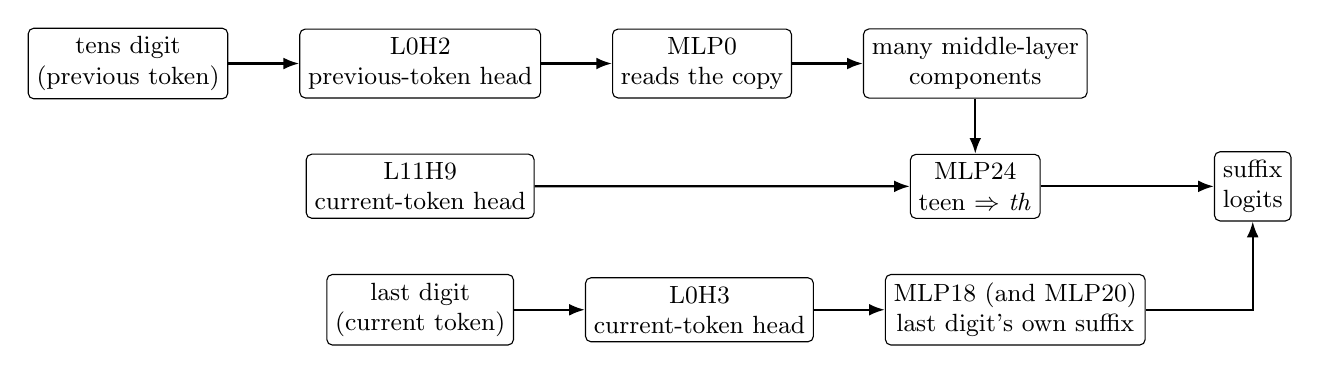
\begin{tikzpicture}[font=\small, node distance=4mm and 9mm,
  box/.style={draw, rounded corners=2pt, align=center, inner sep=3pt, minimum height=7mm},
  arr/.style={-{Latex[length=2mm]}, thick}]
\node[box] (tens) {tens digit\\(previous token)};
\node[box, right=of tens] (h02) {\hd{0}{2}\\previous-token head};
\node[box, right=of h02] (m0) {\mlp{0}\\reads the copy};
\node[box, right=of m0] (mid) {many middle-layer\\components};
\node[box, below=7mm of mid] (m24) {\mlp{24}\\teen $\Rightarrow$ \sfx{th}};
\node[box, below=7mm of h02] (h119) {\hd{11}{9}\\current-token head};
\node[box, right=22mm of m24] (logit) {suffix\\logits};
\node[box, below=7mm of h119] (last) {last digit\\(current token)};
\node[box, right=of last] (h03) {\hd{0}{3}\\current-token head};
\node[box, right=of h03] (m18) {\mlp{18} (and \mlp{20})\\last digit's own suffix};
\draw[arr] (tens) -- (h02); \draw[arr] (h02) -- (m0); \draw[arr] (m0) -- (mid); \draw[arr] (mid) -- (m24);
\draw[arr] (h119) -- (m24); \draw[arr] (m24) -- (logit);
\draw[arr] (last) -- (h03); \draw[arr] (h03) -- (m18); \draw[arr] (m18.east) -| (logit.south);
\end{tikzpicture}
\caption{The path from digits to suffix in \qw{}, as tested in the second round. The teen route (top) is copied early, read by \mlp{0}, spread over many components and gathered at \mlp{24}, which writes a teen override. The last digit's suffix is written separately (bottom); \hd{0}{3}'s role and its route through \mlp{18} rest on exploration and on a separate cross-study test, not on this round's prospective tests. Both routes meet only in the logits.}
\label{fig:path}
\end{figure}

\begin{figure}[t]
\centering
\begin{tikzpicture}
\begin{axis}[width=0.62\linewidth,height=5cm,xlabel={Layer},ylabel={Teen effect read by the logit lens},xmin=0,xmax=28,
  legend style={font=\scriptsize,at={(0.03,0.97)},anchor=north west,draw=none},tick label style={font=\small},label style={font=\small}]
\addplot[thick,black,mark=*,mark size=1.2pt] table[x=layer,y=d4]{fig-lens.dat};
\addlegendentry{4 digits (held out)}
\addplot[thick,gray,dashed,mark=o,mark size=1.2pt] table[x=layer,y=d6]{fig-lens.dat};
\addlegendentry{6 digits (held out)}
\end{axis}
\end{tikzpicture}
\caption{The teen effect as the logit lens reads it at each layer of \qw{}. The decision appears at layer 24, where \mlp{24} writes it; the value at the last layer is the model's own teen effect.}
\label{fig:lens}
\end{figure}

\subsection{\qw{}: what backs up the copy}

When \hd{0}{2} and \hd{1}{6} are removed, a residue of the teen check remains, largest at two digits. Exploration traced it to two later heads that also attend to the previous token, \hd{2}{4} and \hd{5}{2}. Removing them on top of the first pair lowers the teen effect kept below that of every control pair at each length, and most at two digits; on their own they do little (\cref{tab:backup}; S1--S3). Even with all four heads removed, \nv{r2.s.2.ab} of the two-digit teen effect remains, so a further route exists. In exploration, the tens position still held much of the teen information at layers 19--21, which suggests a late second transfer, or a stored pattern for the common two-digit ordinals; neither was tested.

\begin{table}[t]
\centering\small
\caption{\qw{}, held out: teen effect kept after mean ablation at the last position. A = \hd{0}{2} + \hd{1}{6}; B = \hd{2}{4} + \hd{5}{2}; controls are A plus 20 random pairs from layers 2--6.}
\label{tab:backup}
\begin{tabular}{@{}c c c c c c c@{}}
\toprule
Digits & Teen effect & A & A + B & A + random pair & B alone & Drop from adding B \\
\midrule
2 & \nv{r2.s.2.base} & \nv{r2.s.2.a} & \textbf{\nv{r2.s.2.ab}} & \nv{r2.s.2.random_min}--\nv{r2.s.2.random_max} & \nv{r2.s.2.b} & \textbf{\nv{r2.s.2.drop}} \\
3 & \nv{r2.s.3.base} & \nv{r2.s.3.a} & \textbf{\nv{r2.s.3.ab}} & \nv{r2.s.3.random_min}--\nv{r2.s.3.random_max} & \nv{r2.s.3.b} & \nv{r2.s.3.drop} \\
4 & \nv{r2.s.4.base} & \nv{r2.s.4.a} & \textbf{\nv{r2.s.4.ab}} & \nv{r2.s.4.random_min}--\nv{r2.s.4.random_max} & \nv{r2.s.4.b} & \nv{r2.s.4.drop} \\
\bottomrule
\end{tabular}
\end{table}

\subsection{\ol{}: a weak route, not a missing one}

On held-out numbers of three to ten digits the token account of the first round held at every new length (\cref{tab:olmo2}; O3). The teen check is strong where the tens and last digits share a token and weak where the tens digit sits in the previous token, at four, seven and ten digits. At those three lengths, the round-one heads \hd{0}{5}, \hd{0}{0} and \hd{0}{9} carry most of what arrives, and nothing at the in-token lengths (O4). Their effect passes first through \mlp{0} (\nv{r2.o.4.via}, \nv{r2.o.7.via} and \nv{r2.o.10.via} of it, with no other receiver above \nv{r2.o.7.next}; O8).

Two explanations fit a weak check across the boundary: the tens digit may not arrive, or it may arrive and not be used. The evidence favours the first, in a weak form. A linear probe reads teen status at the last token almost perfectly at layer 2 (\nv{r2.o.7.p2}--\nv{r2.o.4.p2}) but less well by layer 15 (\nv{r2.o.10.p15}--\nv{r2.o.4.p15}), while in-token lengths stay at \nv{r2.o.9.p15} or above (O5). The teen direction is small: at every layer its size is at most \nv{r2.o.4.vmax}, \nv{r2.o.7.vmax} and \nv{r2.o.10.vmax} of the three-digit one at four, seven and ten digits, and at least \nv{r2.o.5.vmin} at five digits (O6). The late layers can still use a signal of normal size: adding the three-digit teen direction at layer 8 to non-teen numbers lowers the suffix margin by \nv{r2.o.4.steer}, \nv{r2.o.7.steer} and \nv{r2.o.10.steer} logits at four, seven and ten digits, while random directions of the same size move it by at most \nv{r2.o.4.rand}, \nv{r2.o.7.rand} and \nv{r2.o.10.rand} (O7). The reader works; what reaches it is too faint.

\begin{table}[t]
\centering\small
\caption{\ol{}, held out (96 teen and 96 non-teen numbers per length, plain form). ``Three heads kept'' is the teen effect left after mean-ablating \hd{0}{5}, \hd{0}{0} and \hd{0}{9} at the last position; random triples are from layers 0--2.}
\label{tab:olmo2}
\begin{tabular}{@{}c l c c c c c@{}}
\toprule
Digits & Tokens & Teen effect & AUROC & Three heads kept & Lowest random triple & Probe, layer 2 / 15 \\
\midrule
3 & \nv{r2.o.3.pieces} & \nv{r2.o.3.base} & \nv{r2.o.3.auroc} & \nv{r2.o.3.kept} & \nv{r2.o.3.rmin} & \nv{r2.o.3.p2} / \nv{r2.o.3.p15} \\
4 & \nv{r2.o.4.pieces} & \nv{r2.o.4.base} & \textbf{\nv{r2.o.4.auroc}} & \textbf{\nv{r2.o.4.kept}} & \nv{r2.o.4.rmin} & \nv{r2.o.4.p2} / \textbf{\nv{r2.o.4.p15}} \\
5 & \nv{r2.o.5.pieces} & \nv{r2.o.5.base} & \nv{r2.o.5.auroc} & \nv{r2.o.5.kept} & \nv{r2.o.5.rmin} & \nv{r2.o.5.p2} / \nv{r2.o.5.p15} \\
7 & \nv{r2.o.7.pieces} & \nv{r2.o.7.base} & \textbf{\nv{r2.o.7.auroc}} & \textbf{\nv{r2.o.7.kept}} & \nv{r2.o.7.rmin} & \nv{r2.o.7.p2} / \textbf{\nv{r2.o.7.p15}} \\
8 & \nv{r2.o.8.pieces} & \nv{r2.o.8.base} & \nv{r2.o.8.auroc} & \nv{r2.o.8.kept} & \nv{r2.o.8.rmin} & \nv{r2.o.8.p2} / \nv{r2.o.8.p15} \\
9 & \nv{r2.o.9.pieces} & \nv{r2.o.9.base} & \nv{r2.o.9.auroc} & \nv{r2.o.9.kept} & \nv{r2.o.9.rmin} & \nv{r2.o.9.p2} / \nv{r2.o.9.p15} \\
10 & \nv{r2.o.10.pieces} & \nv{r2.o.10.base} & \textbf{\nv{r2.o.10.auroc}} & \textbf{\nv{r2.o.10.kept}} & \nv{r2.o.10.rmin} & \nv{r2.o.10.p2} / \textbf{\nv{r2.o.10.p15}} \\
\bottomrule
\end{tabular}
\end{table}

\subsection{Other models with one token per digit}

In Qwen3-1.7B-Base, SmolLM2-1.7B and Gemma-4-E2B, heads were picked in exploration by their attention alone: those in layers 0--1 that put at least half of the last token's attention on the previous token (PREV) or on the current token (CUR). In every model, ablating the PREV heads removes part of the teen effect, while random heads from the same layers remove almost none (\cref{tab:other}). Only Qwen3-1.7B has CUR heads by this rule, and they carry the last digit's pull: removing them reverses its sign, while the teen effect is kept. One prediction failed in both of its cells: in Qwen3-1.7B the PREV heads also remove much of the pull (\nv{r2.x.q17.3.PREV.pull} and \nv{r2.x.q17.4.PREV.pull} kept, against the \nv{thr2.X.pull} required). In that model the two kinds of early head divide the work less cleanly than in \qw{}.

\begin{table}[t]
\centering\small
\caption{Other one-token-per-digit models, held out: mean ablation of early heads at the last position. ``Pull'' is the mean suffix margin of non-teen numbers; random sets are 20 sets of the same size from layers 0--1.}
\label{tab:other}
\begin{tabular}{@{}l l c c c c@{}}
\toprule
Model & Heads & Digits & Teen effect kept & Pull kept & Lowest random set \\
\midrule
Qwen3-1.7B-Base & PREV \hd{0}{2}+\hd{1}{6} & 3 / 4 & \nv{r2.x.q17.3.PREV.teen} / \nv{r2.x.q17.4.PREV.teen} & \textbf{\nv{r2.x.q17.3.PREV.pull}} / \textbf{\nv{r2.x.q17.4.PREV.pull}} & \nv{r2.x.q17.3.PREV.rmin} / \nv{r2.x.q17.4.PREV.rmin} (teen) \\
 & CUR \hd{0}{3}+\hd{0}{7} & 3 / 4 & \nv{r2.x.q17.3.CUR.teen} / \nv{r2.x.q17.4.CUR.teen} & \nv{r2.x.q17.3.CUR.pull} / \nv{r2.x.q17.4.CUR.pull} & \nv{r2.x.q17.3.CUR.rmin} / \nv{r2.x.q17.4.CUR.rmin} (pull) \\
SmolLM2-1.7B & PREV \hd{0}{6}+\hd{0}{8} & 3 / 4 & \nv{r2.x.smol.3.PREV.teen} / \nv{r2.x.smol.4.PREV.teen} & \nv{r2.x.smol.3.PREV.pull} / \nv{r2.x.smol.4.PREV.pull} & \nv{r2.x.smol.3.PREV.rmin} / \nv{r2.x.smol.4.PREV.rmin} (teen) \\
Gemma-4-E2B & PREV \hd{0}{4} & 3 / 4 & \nv{r2.x.gemma.3.PREV.teen} / \nv{r2.x.gemma.4.PREV.teen} & \nv{r2.x.gemma.3.PREV.pull} / \nv{r2.x.gemma.4.PREV.pull} & \nv{r2.x.gemma.3.PREV.rmin} / \nv{r2.x.gemma.4.PREV.rmin} (teen) \\
\bottomrule
\end{tabular}
\end{table}

\subsection{A published training run of \ol{} (exploratory)}

Six checkpoints from the first training stage of a published \ol{} training run, already on disk, were run on exploration items (\cref{tab:ckpt}). This analysis is descriptive and was not part of the protocol. The run follows the same recipe as the released model, but the released weights do not descend from it: the released model's token embeddings have cosine \nv{post.lin.emb} with those at the end of this stage, whereas the four published second-stage checkpoints that continue from that point all keep a cosine of at least \nv{post.lin.s2min} (a post hoc comparison, prompted by a companion study). The checkpoints therefore show how this recipe can learn the teen check, not how the released model learnt it. In this run the in-token check forms early. The cross-token check stays near chance until about a trillion tokens and is still weak at the end of the stage. The tens digit can be read at the last token by a probe from early on, but that reading fades with depth, much as in the released model. Ablating the heads at the positions that carry the cross-token route in the released model has no effect at any checkpoint where the effect is large enough to read. Since head positions need not correspond between separately trained models, this shows only that the run does not use those positions in its first stage; it does not date the released model's route.

\begin{table}[t]
\centering\small
\caption{Stage-one checkpoints of a published \ol{} training run of the same recipe, from which the released weights do not descend; exploration items (64 teen and 64 non-teen numbers per length). The three heads are those at the released model's positions \hd{0}{5}, \hd{0}{0} and \hd{0}{9}; their ablation is shown only where the four-digit teen effect is at least \nv{thr2.R1.read} logits.}
\label{tab:ckpt}
\setlength{\tabcolsep}{4.5pt}
\begin{tabular}{@{}r c c c c c c c@{}}
\toprule
 & \multicolumn{4}{c}{Teen AUROC by digits} & \multicolumn{3}{c}{Four digits} \\
\cmidrule(lr){2-5}\cmidrule(l){6-8}
Tokens (billions) & 3 & 4 & 5 & 7 & Teen effect & Three heads kept & Probe, layer 2 / 14 \\
\midrule
1 & \nv{r2.e6.1.auroc3} & \nv{r2.e6.1.auroc4} & \nv{r2.e6.1.auroc5} & \nv{r2.e6.1.auroc7} & \nv{r2.e6.1.base4} & \nv{r2.e6.1.tri} & \nv{r2.e6.1.p2} / \nv{r2.e6.1.p14} \\
21 & \nv{r2.e6.21.auroc3} & \nv{r2.e6.21.auroc4} & \nv{r2.e6.21.auroc5} & \nv{r2.e6.21.auroc7} & \nv{r2.e6.21.base4} & \nv{r2.e6.21.tri} & \nv{r2.e6.21.p2} / \nv{r2.e6.21.p14} \\
84 & \nv{r2.e6.84.auroc3} & \nv{r2.e6.84.auroc4} & \nv{r2.e6.84.auroc5} & \nv{r2.e6.84.auroc7} & \nv{r2.e6.84.base4} & \nv{r2.e6.84.tri} & \nv{r2.e6.84.p2} / \nv{r2.e6.84.p14} \\
420 & \nv{r2.e6.420.auroc3} & \nv{r2.e6.420.auroc4} & \nv{r2.e6.420.auroc5} & \nv{r2.e6.420.auroc7} & \nv{r2.e6.420.base4} & \nv{r2.e6.420.tri} & \nv{r2.e6.420.p2} / \nv{r2.e6.420.p14} \\
1{,}007 & \nv{r2.e6.1007.auroc3} & \nv{r2.e6.1007.auroc4} & \nv{r2.e6.1007.auroc5} & \nv{r2.e6.1007.auroc7} & \nv{r2.e6.1007.base4} & \nv{r2.e6.1007.tri} & \nv{r2.e6.1007.p2} / \nv{r2.e6.1007.p14} \\
4{,}001 & \nv{r2.e6.4001.auroc3} & \nv{r2.e6.4001.auroc4} & \nv{r2.e6.4001.auroc5} & \nv{r2.e6.4001.auroc7} & \nv{r2.e6.4001.base4} & \nv{r2.e6.4001.tri} & \nv{r2.e6.4001.p2} / \nv{r2.e6.4001.p14} \\
\bottomrule
\end{tabular}
\end{table}

%======================================================================
\section{Discussion}
\label{sec:discussion}

\paragraph{The picture across both rounds.} In \qw{}, applying the teen exception takes three steps. An early, general-purpose head copies the previous digit to the last position. \mlp{0} reads it there at once. The resulting signal is spread over many components and gathered again at \mlp{24}, which writes a teen override towards \sfx{th}. A separate early route and \mlp{18} write the suffix that the last digit alone calls for, and the two meet only in the logits: the override does not consult the last digit, and the last-digit writer does not consult the tens digit. Backup heads further on can do part of the copying, mostly for two-digit numbers. In \ol{}, the copying step is needed only when the tokeniser has separated the two digits. Where it is needed, it delivers a signal too faint for the late layers to act on reliably, although they act on a signal of normal size. That is where the model makes its teen errors, and a thousands separator removes them by putting both digits in one token. This fits the finding of \citet{singh2024tokenization} that comma-separated numbers help large models with arithmetic, and gives one concrete reason: a separator can put the digits that a rule needs into one token.

\paragraph{General parts and task parts.} A separate cross-study test in the same project (unpublished) asked whether components found in several of our studies are shared. On held-out text it found that \hd{0}{2} behaves as a general previous-token head and \hd{0}{3} as a general current-token head, both used by other tasks, and that \hd{11}{9} is a suffix head. The teen check therefore has no dedicated early head. It uses a general previous-token mover, the kind of early head that induction heads also build on~\citep{olsson2022induction}, and the task-specific work happens in the MLPs that read and decide. That early previous-token heads also carry part of the check in three further models with one token per digit suggests the arrangement is common. The weaker separation of roles in Qwen3-1.7B, where the previous-token heads also carry much of the pull, shows that its details vary.

\paragraph{What the results do not show.} The accounts are partial. Even with both pairs of copying heads removed, \nv{r2.s.2.ab} of the two-digit teen effect remains, and we did not find the route that carries it. Between \mlp{0} and \mlp{24} the signal is spread thinly, and we did not trace its individual carriers. We traced the path only in \qw{}; in the other models we tested the early heads alone. In \ol{} we did not find which late components fail to read the faint cross-token signal. The checkpoint analysis is exploratory, covers only the first stage of a published training run, and that run is not the one the released weights come from, so it cannot say when the released model's route formed. The frame-dependent errors of \qw{} noted in \cref{sec:explore} remain unexplained. The GPT-2 and Pythia-1B results rest on ten numbers each, and their internals were not studied.

\paragraph{Scope.} Base models under two billion parameters, English frames, numbers up to ten digits, and a choice among four suffix tokens at one position. Mean ablation replaces a component's output with an average that need not occur on any real input; direct attribution linearises the final normalisation; and methodological choices in patching and ablation can change which components appear important~\citep{heimersheim2024patching,zhang2024patching}. The random-set controls bound but do not remove these concerns. Three- to five-digit numbers in the second round's held-out set had been read in the first round, in other frames.

\paragraph{Process.} In both rounds, thresholds were set from exploration and were not changed after the run, and no output of either test was rerun. In the second round, every test except those on the further models was first run once on exploration items. Two thresholds were reset from that run, and a third (for the further models) from the last exploration run, all before the freeze. A dated amendment to the second charter moved the freeze later than planned, let one exploration run that was already queued finish, and allowed the checkpoint analysis to be completed as a descriptive result; no held-out material was read before the freeze. The second round's held-out date frames remain unread. Post hoc analyses are limited to two from the first round (the make-up of the GPT-2 and Pythia-1B boundary sets, and exploration AUROCs recomputed with ties counted as one half) and to the descriptive checkpoint analysis above, together with the weight comparison that places those checkpoints in a different run from the released model.

\paragraph{Use of language-model assistants.} Language-model assistants were used to write analysis code, run the experiments and draft this text under the author's direction. All numbers are generated from saved outputs and checked by script.

\bibliographystyle{plainnat}
\bibliography{refs}

\end{document}
